\documentclass[a4paper,12pt]{article}
\usepackage[italian]{babel}

% immagini
\usepackage{graphicx}
\usepackage{svg}
\usepackage{amsthm}
\usepackage{geometry}
\usepackage{subcaption}
% matematica
\usepackage{amsmath}
\usepackage{amsfonts}
\usepackage{unicode-math}

% codice
\usepackage{listings}
\lstset{
    basicstyle=\small\ttfamily,
    numbers=left,
    numberstyle=\small\ttfamily
}

% \usepackage{blindtext}
\usepackage{titlesec}
% \usepackage{geometry}
% \usepackage{relsize}
\usepackage{tikz}
% \geometry{
% a4paper,
% total={190mm,257mm},
% left=25mm,
% right=25mm,
% top=50mm,
% }
\geometry{a4paper, margin=1in} % Set margins to fit the entire content better
\usepackage{hyperref}

% \sloppy % ?

% comandi per riferirsi agli algoritmi
\newcommand{\QuickSelect}{\textsc{QuickSelect}}
\newcommand{\HeapSelect}{\textsc{HeapSelect}}
\newcommand{\MoMSelect}{\textsc{MoMSelect}}

% comandi per la notazione asintotica
\newcommand{\Tquad}{\ifmmode \Theta(n^2) \else $\Theta(n^2)$\fi} % Θ(n^2)
\newcommand{\Tlin}{\ifmmode \Theta(n) \else $\Theta(n)$\fi} % Θ(n)
\newcommand{\Olin}{\ifmmode O(n) \else $O(n)$\fi} % O(n)

\begin{document}

\begin{titlepage} % pagina riservata al titolo
    \begin{center}
        \vspace*{1cm}
        {\Huge\bfseries Analisi di algoritmi di selezione\par}
        \vspace{.5cm}
        {\LARGE Progetto di laboratorio di Algoritmi e Strutture Dati\par}
        \vspace{1cm}
        \begin{figure}[h]
            \centering
            
\includegraphics[width=.5\textwidth]{photo/uniud_logo.png}
        \end{figure}
        \vspace{1.5cm}
        {\LARGE Università degli studi di Udine\par}
        {\LARGE Dipartimento di scienze Informatiche, Matematiche e Fisiche\par}
        \vspace{.5cm}
        {\Large Anno Accademico 2023/2024\par}
        \vfill
	    {\Large \textit{Ludovico Gerardi} (mat. 162367) - \texttt{162367@spes.uniud.it} \par}
	    {\Large \textit{Lorenzo Sclauzero} (mat. 162013) - \texttt{162013@spes.uniud.it} \par}
	    {\Large \textit{Riccardo Pantanali} (mat. 162473) - \texttt{162473@spes.uniud.it} \par}
    \end{center}
\end{titlepage}



\section{Introduzione}
Il progetto ha come scopo l'implementazione di tre algoritmi di selezione e l'analisi della loro complessità.
Dato un vettore di interi $v$ di dimensione $n$ e un intero $k$ con $1 < k \le n$, gli algoritmi di selezione calcolano il $k$-esimo elemento più piccolo di $v$.

I tre algoritmi discussi sono \QuickSelect{}, \HeapSelect{} e \MoMSelect{} (che sta per median-of-medians select); vengono presentati nella sezione \ref{sec:presentazione-algoritmi} insieme all'algoritmo utilizzato per la generazione dell'input.
Nella sezione \ref{sec:misurazione} si discute brevemente la misurazione dei tempi di esecuzione, necessaria per l'analisi della complessità.
Nella sezione \ref{sec:grafici} vengono presentati e discussi i risultati delle misurazioni sotto forma di grafici.
Infine nella sezione \ref{sec:confronto-mom} viene proposto un confronto tra due varianti di \MoMSelect{}.



\section{Presentazione degli algoritmi}
\label{sec:presentazione-algoritmi}

\subsection{Algoritmi di selezione}
\paragraph{\QuickSelect}
Questo algoritmo partiziona iterativamente $v$ rispetto a un elemento scelto come pivot e confronta la posizione finale del pivot con $k$: se sono uguali allora l'algoritmo termina, ritornando $v[k]$; altrimenti la prossima iterazione si restringe alla partizione sinistra o destra di $v$, a seconda che $k$ sia rispettivamente minore o maggiore della posizione finale del pivot.
Quest'ultimo viene scelto sempre come l'ultimo elemento del sottovettore considerato.
Così facendo la complessità nel caso peggiore è \Tquad{} (quando il vettore è già ordinato, in un senso o nell'altro), mentre nel caso medio è \Tlin.

Al netto del caso peggiore, come si vedrà il basso overhead dovuto alla scelta del pivot porta a un vantaggio rispetto agli altri algoritmi di selezione, e soprattutto rispetto a \MoMSelect{}, che ha la stessa complessità di \QuickSelect{} nel caso medio.

L'implementazione è stata fatta in modo iterativo e non ricorsivo per evitare di effettuare troppe chiamate ricorsive nel caso peggiore e quindi incorrere in errore in tal senso.

\paragraph{\HeapSelect}
L'algoritmo sfrutta due heap $H_1$ e $H_2$.
$H_1$ è una min-heap che viene costruita a partire da $v$ in tempo lineare e non viene successivamente modificata, mentre $H_2$ è una min-heap che inizialmente contiene solo il nodo radice di $H_1$.
Ad ogni iterazione viene estratta la radice $r$ da $H_2$ e vengono aggiunti i figli di $r$ in $H_1$ all'interno di $H_2$.
Dopo $k-1$ iterazioni $r$ è l'elemento cercato, cioè il $k$-esimo più piccolo all'interno di $v$.
Siccome cercare il $k$-esimo elemento più piccolo equivale a cercare l'elemento $(n-k+1)$-esimo più grande, se $k>n/2$ si utilizza una max-heap per $H_2$, il che consente di ridurre il numero di iterazioni necessarie.
Questo algoritmo ha una complessità temporale pari a $O(n+k\log k)$.
Essendo $1 \le k \le n$, la complessità effettiva varia da $O(n)$ a $O(n\log n)$; nella sezione \ref{sec:grafici} si analizzano entrambi i casi.

\paragraph{\MoMSelect}
<<<<<<< HEAD
Il funzionamento ad alto livello di \MoMSelect{} è come quello di \QuickSelect: iterare sulla porzione di vettore che contiene l'elemento cercato.
La differenza tra i due algoritmo sta nella scelta del pivot.
Infatti $MomSelect$ effettua una chiamata ricorsiva ulteriore per trovare la mediana delle mediane, ovvero divide il vettore in blocchi da $5$ elementi (eccetto al più l'ultimo blocco), ordina poi ciascun blocco e ne calcola la mediana, quindi effettua una chiamata ricorsiva sulle mediane appena calcolate per trovarne la mediana, ovvero impostando $k=m/2$, dove $m$ è il numero delle mediane calcolate.
=======
Il funzionamento ad alto livello di \MoMSelect{} è come quello di \QuickSelect: restringersi alla porzione di vettore che contiene l'elemento cercato.
La differenza tra i due algoritmi sta nella scelta del pivot.
Infatti \MoMSelect{} effettua una chiamata ricorsiva per trovare la mediana delle mediane, ovvero divide il vettore in blocchi da $5$ elementi (eccetto al più l'ultimo blocco), ordina poi ciascun blocco e ne calcola la mediana, quindi effettua una chiamata ricorsiva sulle sul nuovo vettore appena calcolato per trovarne la mediana; in tale chiamata ricorsiva $k=m/2$, dove $m=\lceil n/5\rceil$ è il numero delle mediane calcolate.
Una volta trovata la mediana delle mediante la utilizza come pivot nel partizionamento del vettore principale.
>>>>>>> c06742b94e506bd4ed1f0863dd0aedfdc00b8d45
Sono proposte due varianti:
\begin{enumerate}
    \item non in-place: alloca un nuovo vettore ad ogni chiamata ricorsiva per memorizzare le mediane dei blocchi;
    \item quasi in-place: riutilizza lo spazio allocato per il vettore originariamente fornito in input; nello specifico: utilizza le prime $m$ posizioni.
\end{enumerate}
In entrambi i casi, la complessità temporale dell'algoritmo è \Tlin{}.
Nei grafici della sezione \ref{sec:grafici} verrà utilizzata la versione quasi in-place.


\subsection{Algoritmo per la generazione dei vettori}
La lunghezza $n$ dei vettori generati varia da $n_{\min}=10^2$ a $n_{\max}=10^5$, mentre i valori degli interi generati variano da $0$ a $10^5$.
In tutte le misurazioni, eccetto quella con $n$ fissato, la lunghezza dei vettori cresce secondo la serie geometrica
\[
    L(i) = n_{\min} \cdot \left(\frac{n_{\max}}{n_{\min}}\right)^{i/99}
\]
dove $i$ è il numero dell'iterazione corrente, che varia da $0$ a $99$, per un totale di $100$ iterazioni.
Si noti in particolare che $L(0) = n_{\min}$ e $L(99) = n_{\max}$.

Vi è anche un'altra procedura per la generazione di un vettore, utilizzata per il caso peggiore di \QuickSelect{}, che genera pseudocasualmente un vettore e poi lo ordina in modo crescente.


\section{Misurazione dei tempi di esecuzione}
\label{sec:misurazione}
La misurazione dei tempi necessari per calcolare il $k$-esimo elemento in un vettore viene effettuata considerando la lunghezza \( n \) di $v$ vettore di input e l'errore relativo massimo, fissato a $e_{\max} = 10^{-3}$.
Per ogni $n$, gli algoritmi implementati ripetono il calcolo un numero di volte tale da garantire un errore massimo relativo pari a  $e_{\max}$, assicurando così un tempo totale maggiore o uguale a \( T_{\min} \), calcolato come \[ T_{\min} = R \left( \frac{1}{e_{\max}} + 1 \right) \] dove \( R \) rappresenta la risoluzione del clock.
Il tempo totale così ottenuto viene diviso per il numero di volte che l'algoritmo ha eseguito.

Inoltre prima e dopo il codice che effettua la misurazione sono state inserite istruzioni per disabilitare e successivamente riabilirare il \emph{garbage collector} di Python, in modo da non incorrere in errori di misurazione dovuti ad esso.


\newpage

\section{Rappresentazione grafica dei risultati}
\label{sec:grafici}

\subsection{Caso $k=n/2$}
\begin{figure}[h]
            \centering
            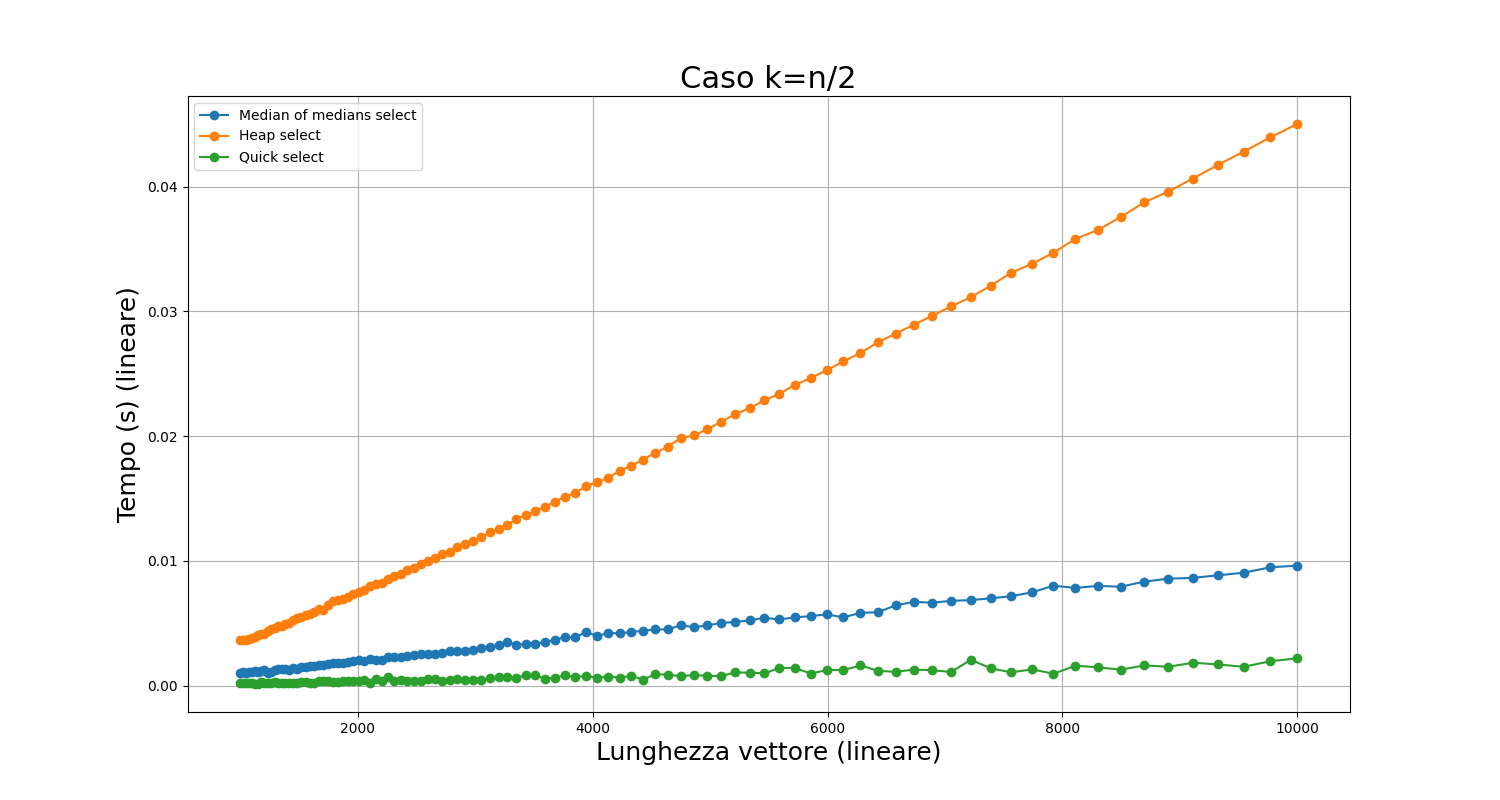
\includegraphics[width=.83\textwidth]{graphs/k_const_n.png}
            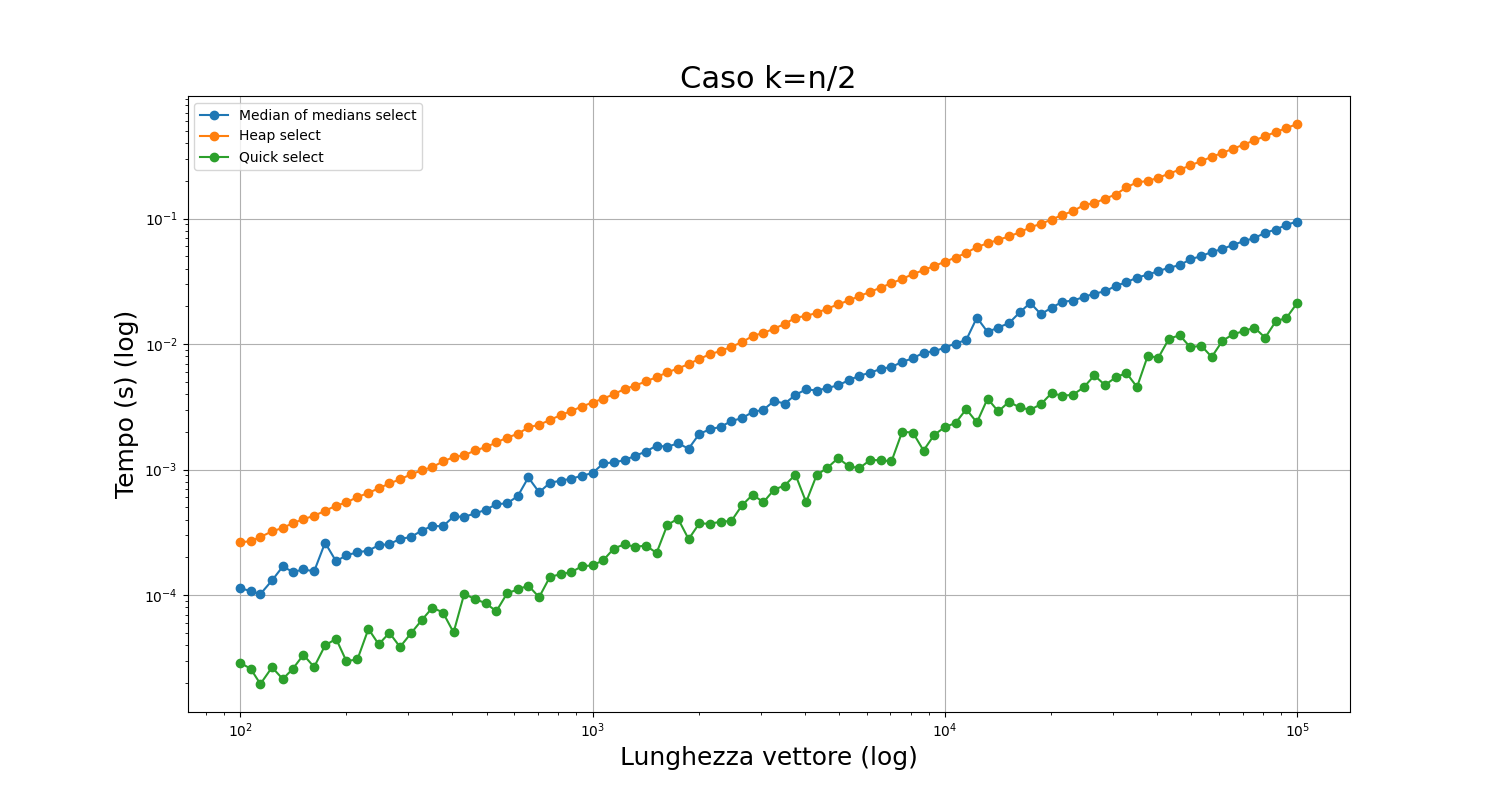
\includegraphics[width=.83\textwidth]{graphs/k_const_2xlog.png}
\end{figure}
Come è evidenziato dai grafici, nel caso in cui $k=n/2$ l'algoritmo \HeapSelect{} è più inefficiente rispetto a \QuickSelect{} e \MoMSelect{}.
Per spiegare questo comportamento occorre tenere conto della complessità di \HeapSelect{}; infatti sostituendo $k$ con $n/2$ nella formula della complessità di ottiene:
\[\begin{split}
	O(n + k\log k) 	& = O\left(n + \frac{n}{2}\log \frac{n}{2}\right) \\
			& = O\left(n + \frac{n}{2}(\log n - \log 2)\right) \\
			& = O\left(n + \frac{n}{2}\log n - \frac{n}{2}\log 2\right) \\
			& = O(n \log n)
\end{split}\]
cioè la crescita di \HeapSelect{} risulta superlineare.
È facile vedere che lo stesso risultato si ottiene ogni volta che $k$ è una frazione di $n$.

Invece \MoMSelect{} e \QuickSelect{} hanno entrambi complessità $O(n)$.
Tuttavia \QuickSelect{} risulta più veloce rispetto a \MoMSelect{}, ciò è dovuto all'overhead richiesto da quest'ultimo algoritmo per calcolare la mediana delle mediane.

\subsection{Caso $k$ estremo}
\begin{figure}[h]
            \centering
            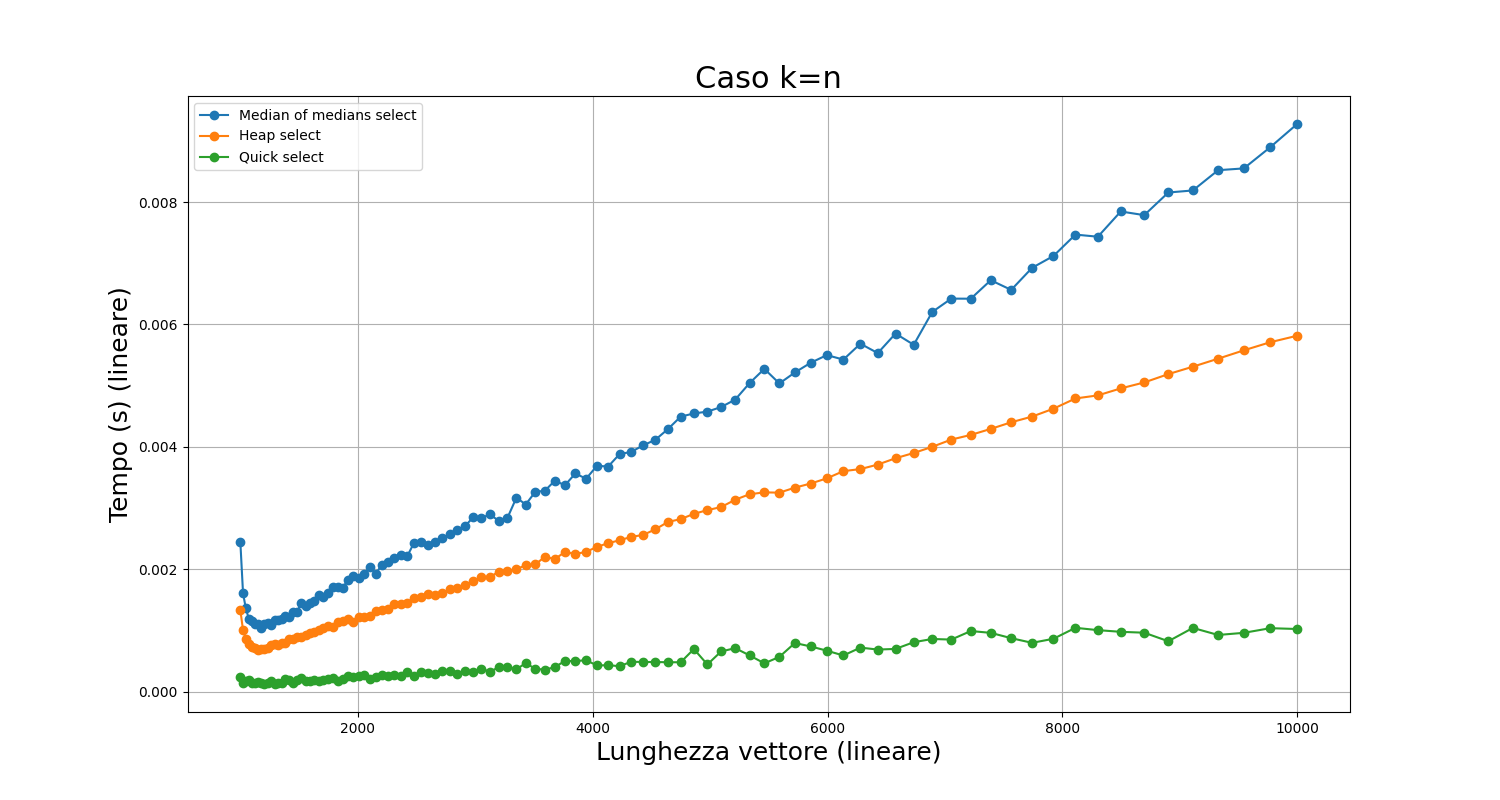
\includegraphics[width=.83\textwidth]{graphs/k_last_n.png}
            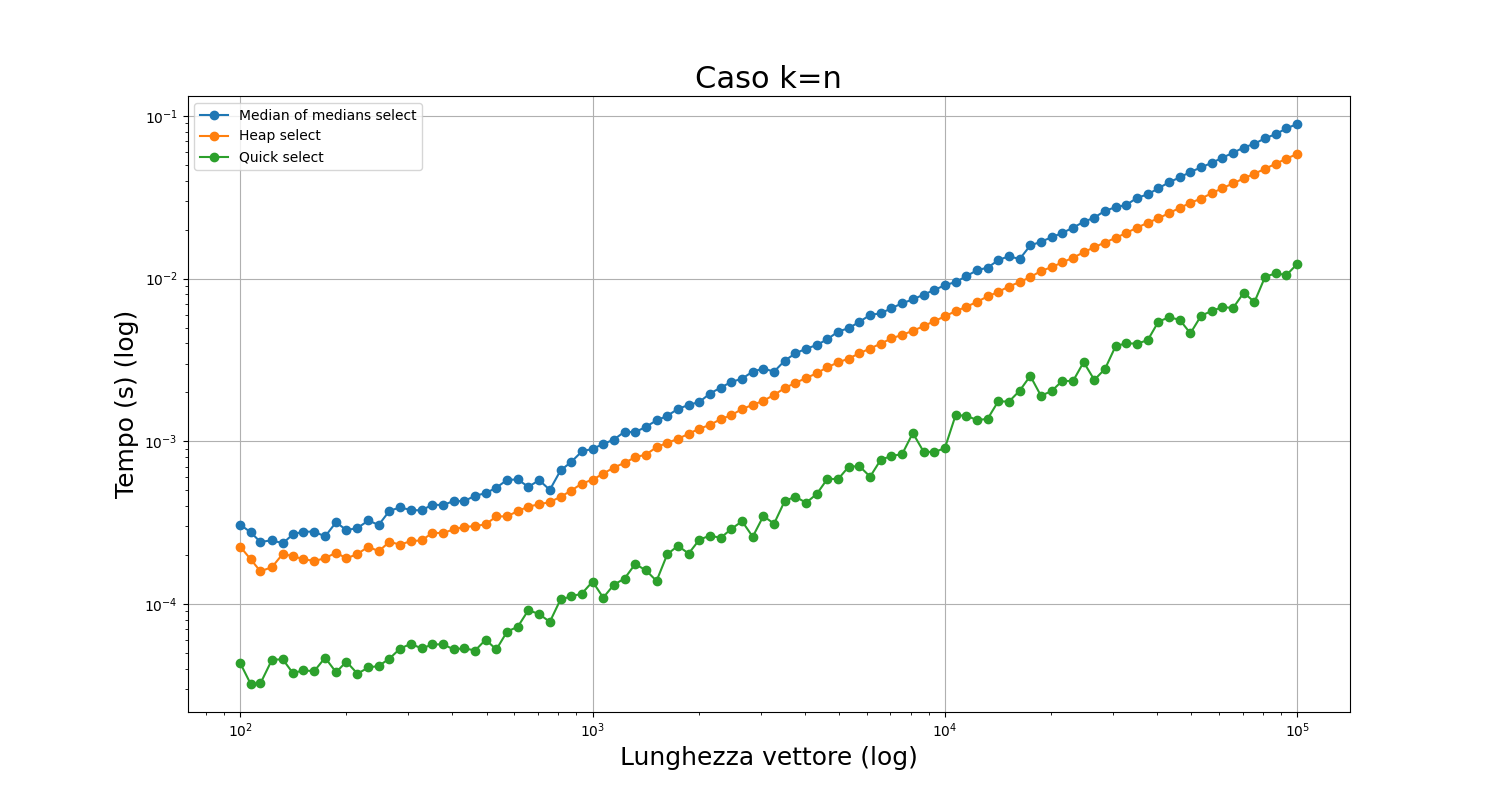
\includegraphics[width=.83\textwidth]{graphs/k_last_2xlog.png}
\end{figure}
Nel caso in cui $k$ sia un estremo del vettore, cioè $k=1$ o $k=n$, si nota un netto miglioramento da parte di \HeapSelect{}, tanto da diventare migliore di \MoMSelect{}.
Infatti, dato che $k$ è costante, il contributo del fattore $k\log k$ diventa trascurabile e quindi il costo di \HeapSelect{} diventa $O(n)$; tale costo è per la maggior parte dovuto alla costruzione dell'heap.
Possiamo quindi affermare che questa operazione risulta più veloce, seppure di poco, rispetto al calcolo della mediana della mediane.

Per quanto riguarda \QuickSelect{} e \MoMSelect{}, il loro andamento risulta praticamente invariato rispetto al caso precedente.
\QuickSelect{} risulta ancora l'algoritmo più efficiente.


\newpage
\subsection{Caso $k$ random}
\begin{figure}[h]
            \centering
            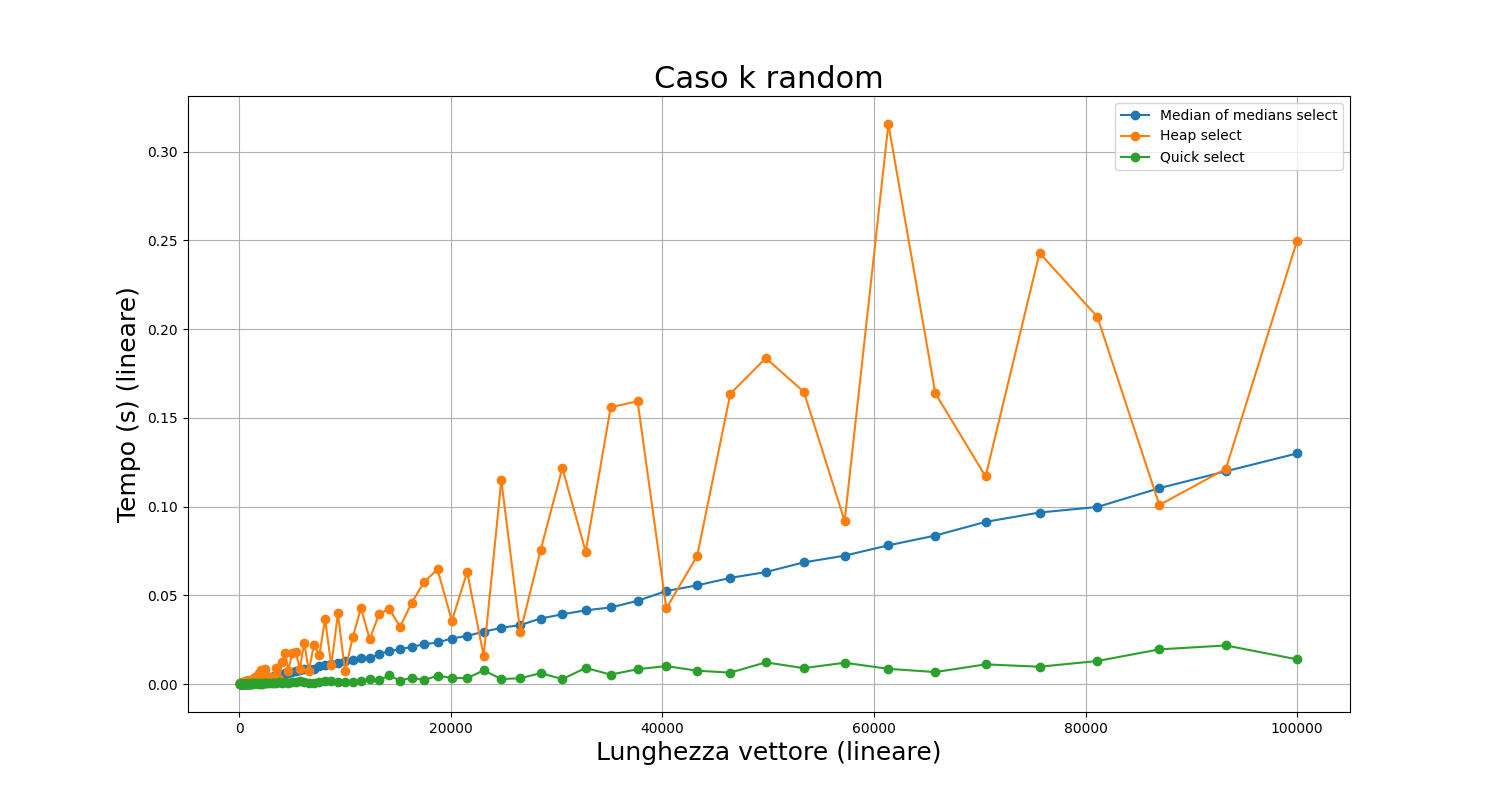
\includegraphics[width=.83\textwidth]{graphs/k_random_n.png}
            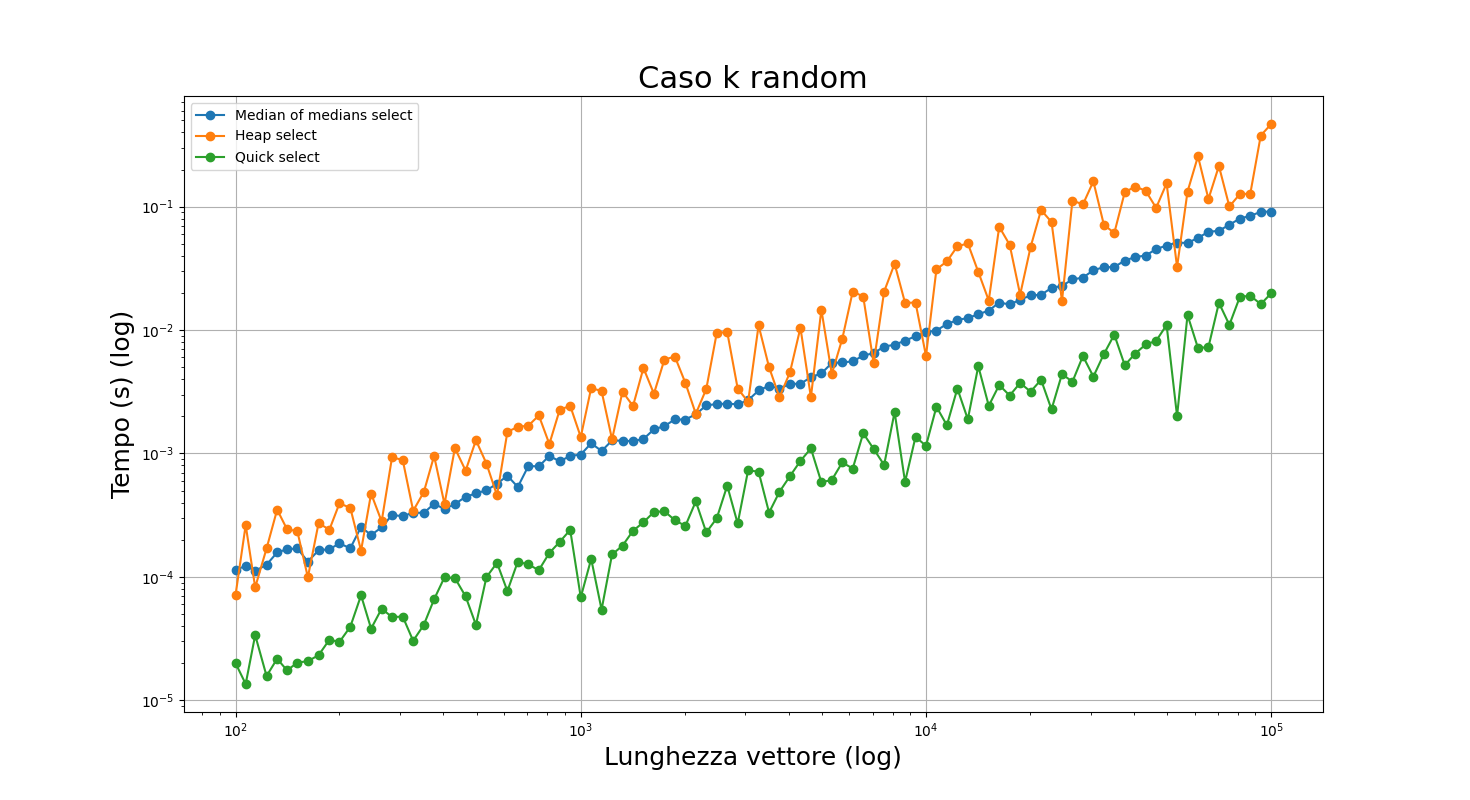
\includegraphics[width=.83\textwidth]{graphs/k_random_2xlog.png}
\end{figure}

Nel caso in cui $k$ sia casuale emerge chiaramente l'indipendenza dell'algoritmo \MoMSelect{} da $k$: il suo andamento risulta infatti molto stabile al variare di $k$, e ciò è da attribuirsi al calcolo della mediana delle mediane, che assicura un andamento lineare.
Invece \HeapSelect{} mostra un andamento più instabile.
Ciò è dovuto al fatto che $k$ determina la sua complessità, che varia da $O(n)$ a $O(n\log n)$, come si è già visto.
Anche \QuickSelect{} si mostra più instabile di \MoMSelect{}.
Ricordiamo infatti che nel caso peggiore la complessità di \QuickSelect{} è $\Theta(n^2)$.



\newpage
\subsection{Caso $n$ fissato e $k$ variato}
\begin{figure}[h]
    \centering
    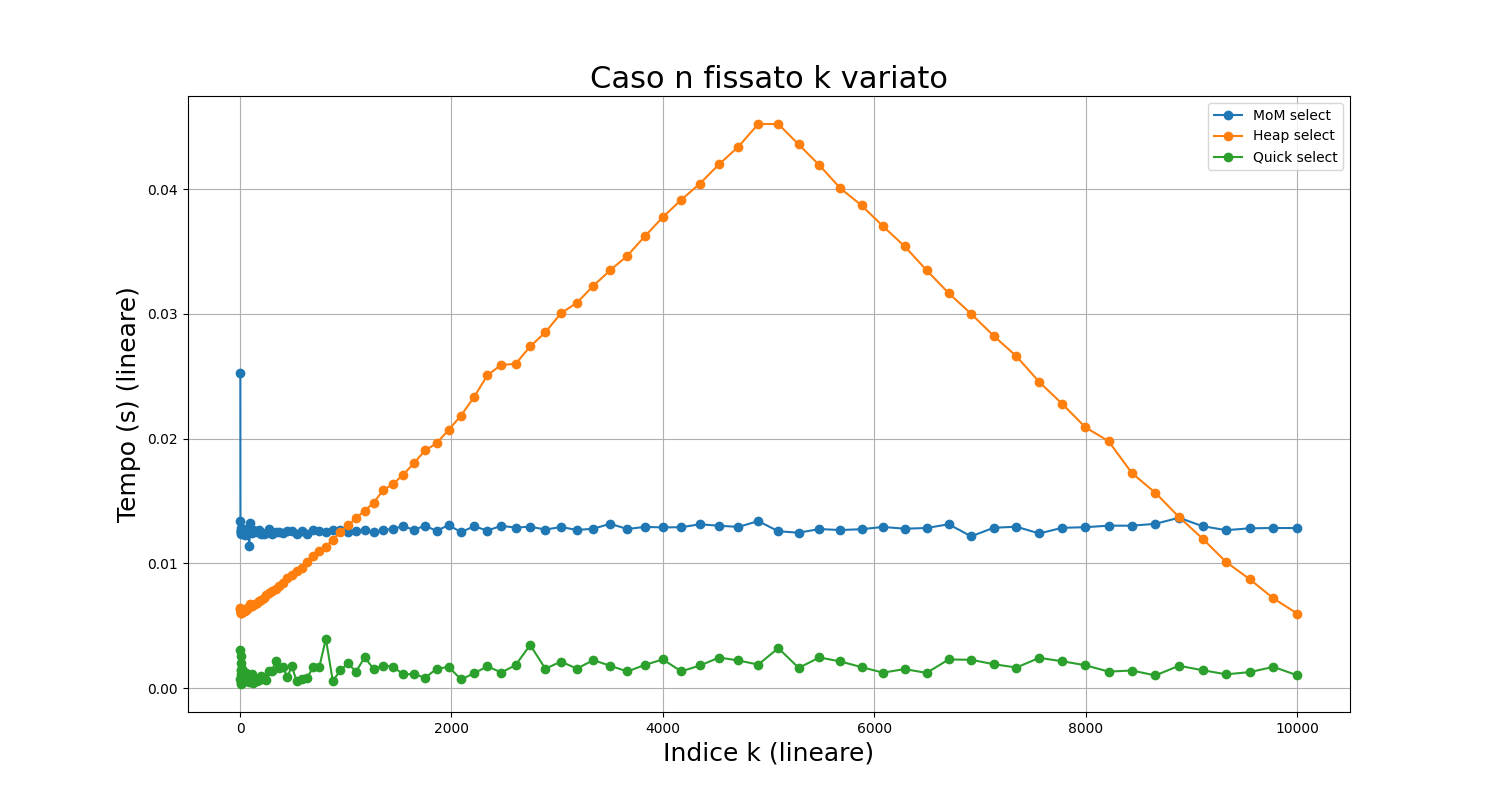
\includegraphics[width=.83\textwidth]{graphs/n_fixed_n.png}
    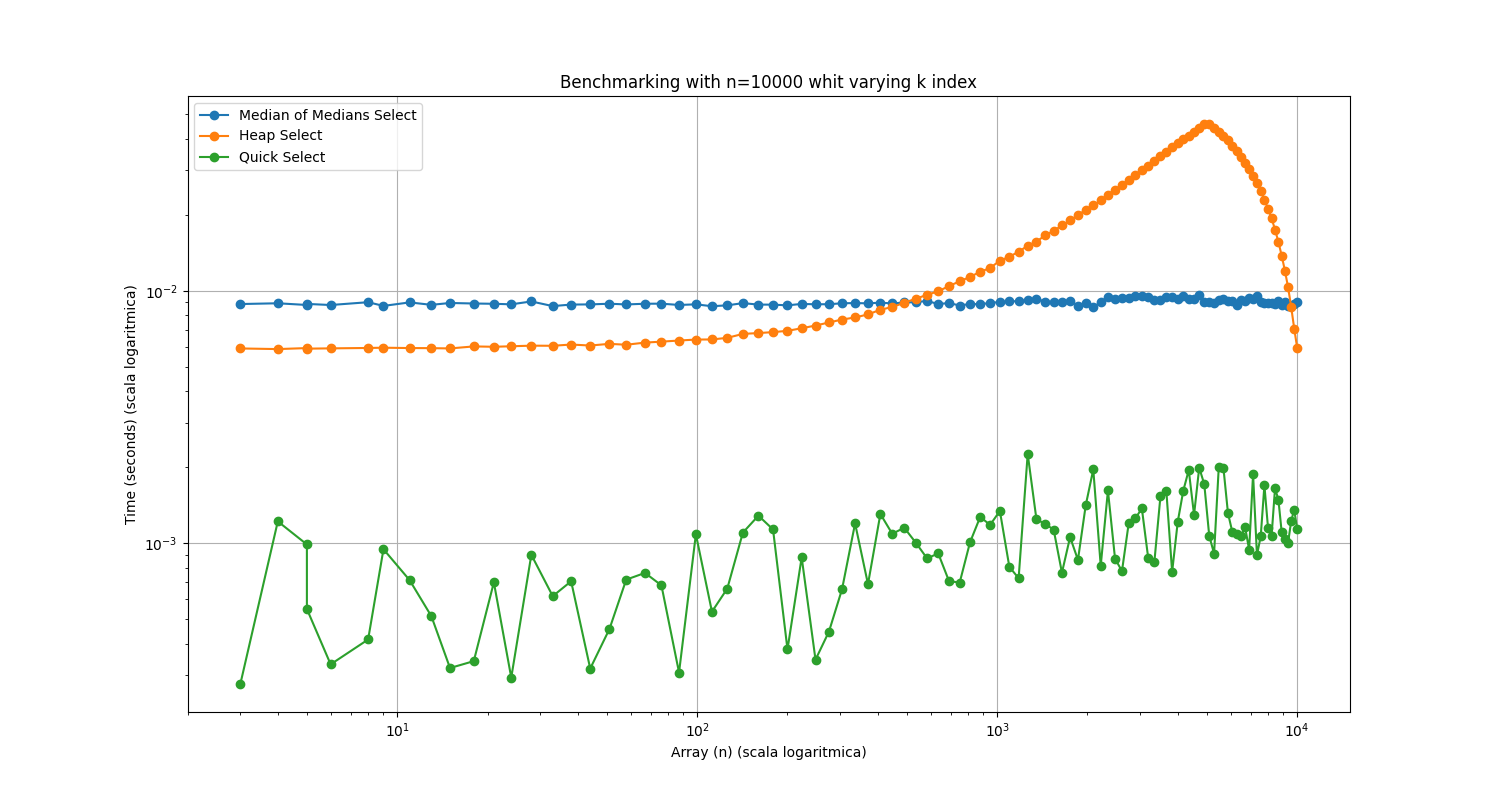
\includegraphics[width=.83\textwidth]{graphs/n_fixed_2xlog.png}
\end{figure}

In questo caso la lunghezza di $n$ è fissata a $10000$ e $k$ varia nell'intervallo $[1,\dots,10000]$.
Risulta evidente la dipendenza di \HeapSelect{} dallo stesso: il suo andamento piramidale mostra come tempo di esecuzione cresce monotonicamente fino a $k=n/2$ e poi decresce monotonicamente.
Ciò è naturalmente dovuto al fatto che l'implementazione utilizza una max heap per $k>n/2$; se non fosse così è facile immaginare che il tempo continuerebbe a crescere dopo $n/2$.

Riguardo a \QuickSelect{} e \MoMSelect{} non traspare nulla di differente da quello che abbiamo già evidenziato nelle sezioni precedenti.

\newpage
\subsection{Caso peggiore per \QuickSelect}

Dai casi precedenti si è visto come \QuickSelect{}, nonostante abbia nel caso peggiore una complessità $\Tquad$, difatto con un vettore generato pseudo-casualemente risulti essere migliore di \HeapSelect{} e \MoMSelect{}, e quindi può essere un buon candidato come algoritmo di selezione se si è ragionevolmente sicuri che il caso peggiore non possa verificarsi.
Ma vediamo ora un caso in cui ciò può accadere, cioè quando il vettore è ordinato in modo crescente e $k=1$, ovvero quello rappresentato nei grafici di seguito.
(Nota: a differenza degli altri grafici, nei seguenti la dimensione massima del vettore è stata fissata a $10000$ per non prolungare troppo i tempi richiesti alla misurazione.)

\begin{figure}[h]
    \centering
    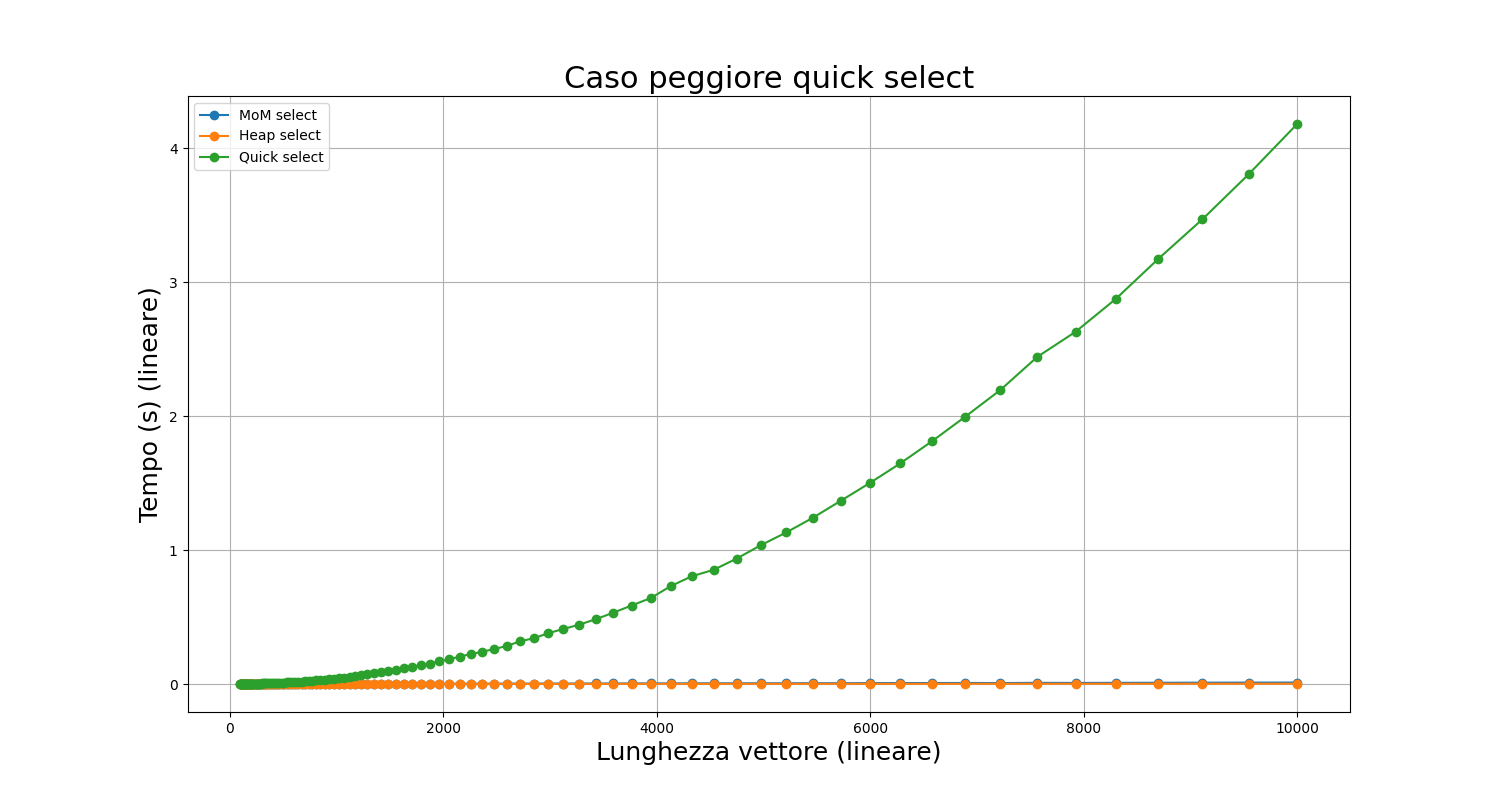
\includegraphics[width=.83\textwidth]{graphs/QS_n.png}
    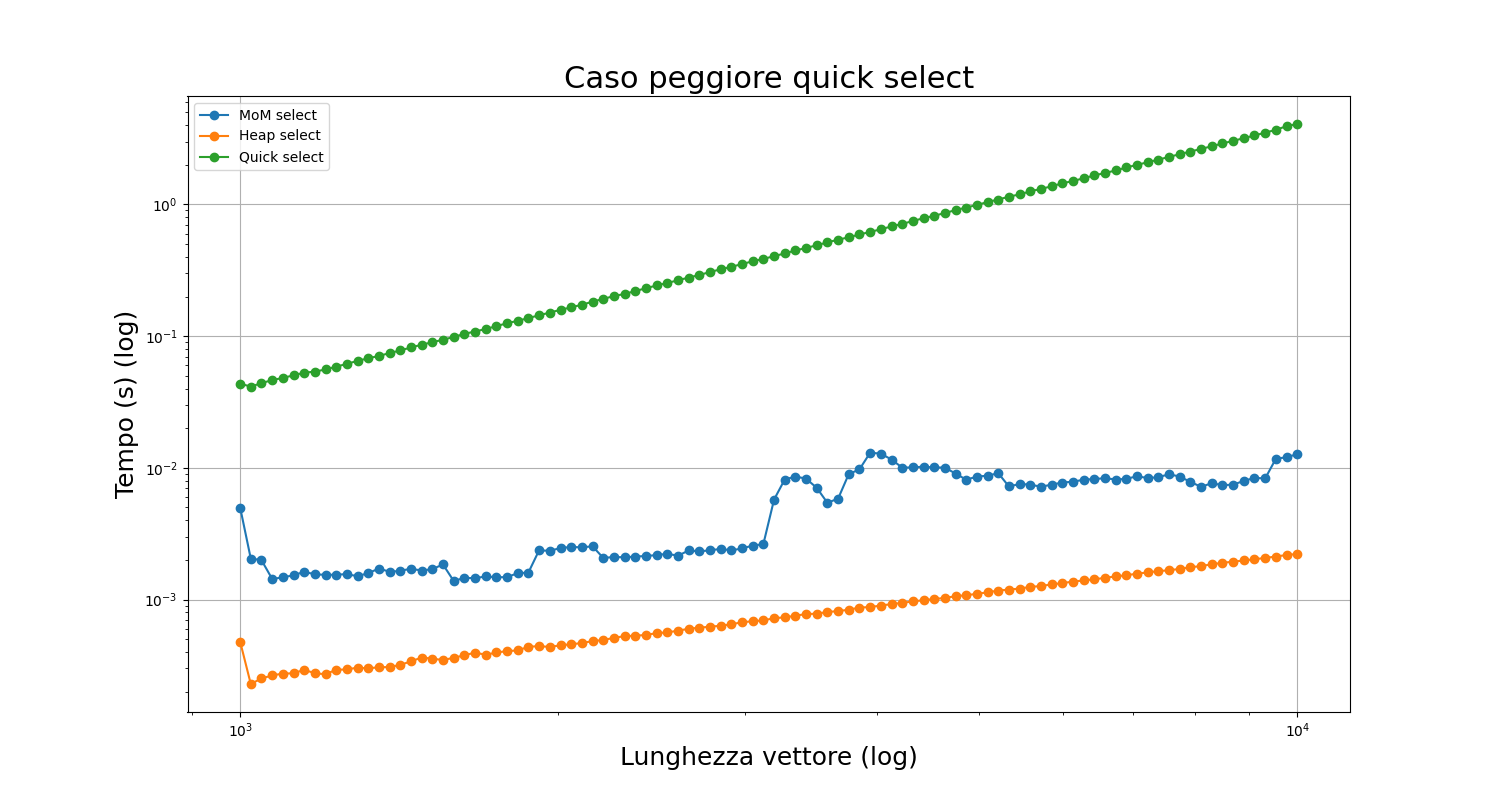
\includegraphics[width=.83\textwidth]{graphs/QS_2xlog.png}
\end{figure}

Nel primo grafico si vede chiaramente l'andamento quadratico di \QuickSelect{}, che al crescere di $n$ si discosta enormemente dagli andamenti di \HeapSelect{} e \MoMSelect{}.
Anche dal grafico logaritmico si nota che, mentre \HeapSelect{} e \MoMSelect{} sono paralleli, la retta di \QuickSelect{} ha un coefficiente angolare maggiore degli altri due, e di conseguenza il comportamento asintotico è superlineare.

C'è anche un secondo caso peggiore per \QuickSelect{}, che però l'implementazione qui proposta non permette di osservare.
Si tratta del caso in cui il vettore è ordinato in modo crescente, $k=n$ e il pivot è selezionato sempre come il primo elemento del sottovettore considerato.
La nostra implementazine non lo permette in quanto il pivot è selezionato sempre come l'ultimo elemento del vettore.



\section{Confronto tra MoM}
\label{sec:confronto-mom}
Proponiamo infine un confronto con $k$ fissato a $n/2$ tra due varianti di \MoMSelect{}, che differiscono per lo spazio utilizzato: ricordiamo che la variante non in-place alloca un nuovo vettore per memorizzare le mediane calcolate, mentre la variante quasi in-place riutilizza le prima $m$ posizione del vettore originale.

\begin{figure}[h]
    \centering
    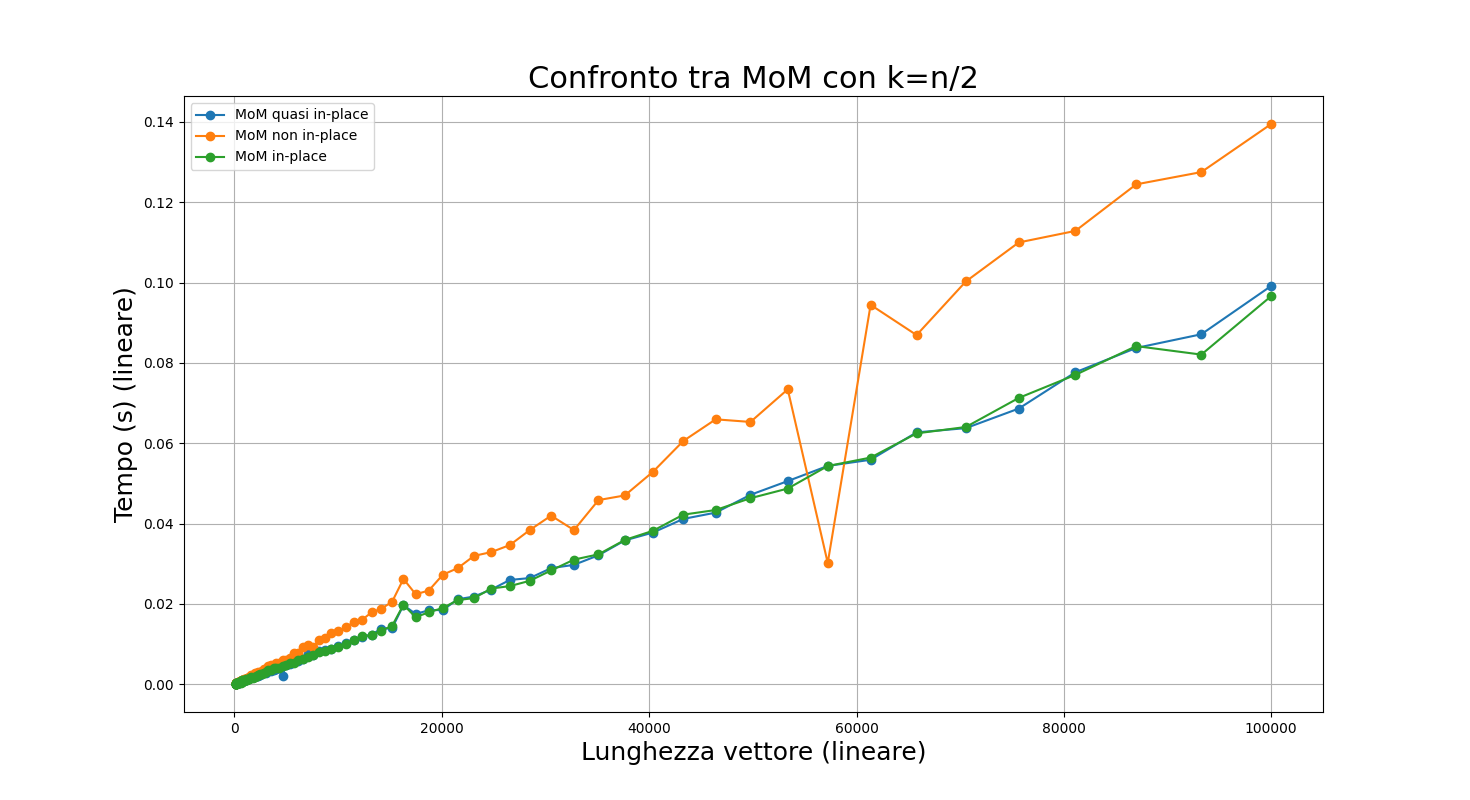
\includegraphics[width=.83\textwidth]{graphs/MoMs_n.png}
    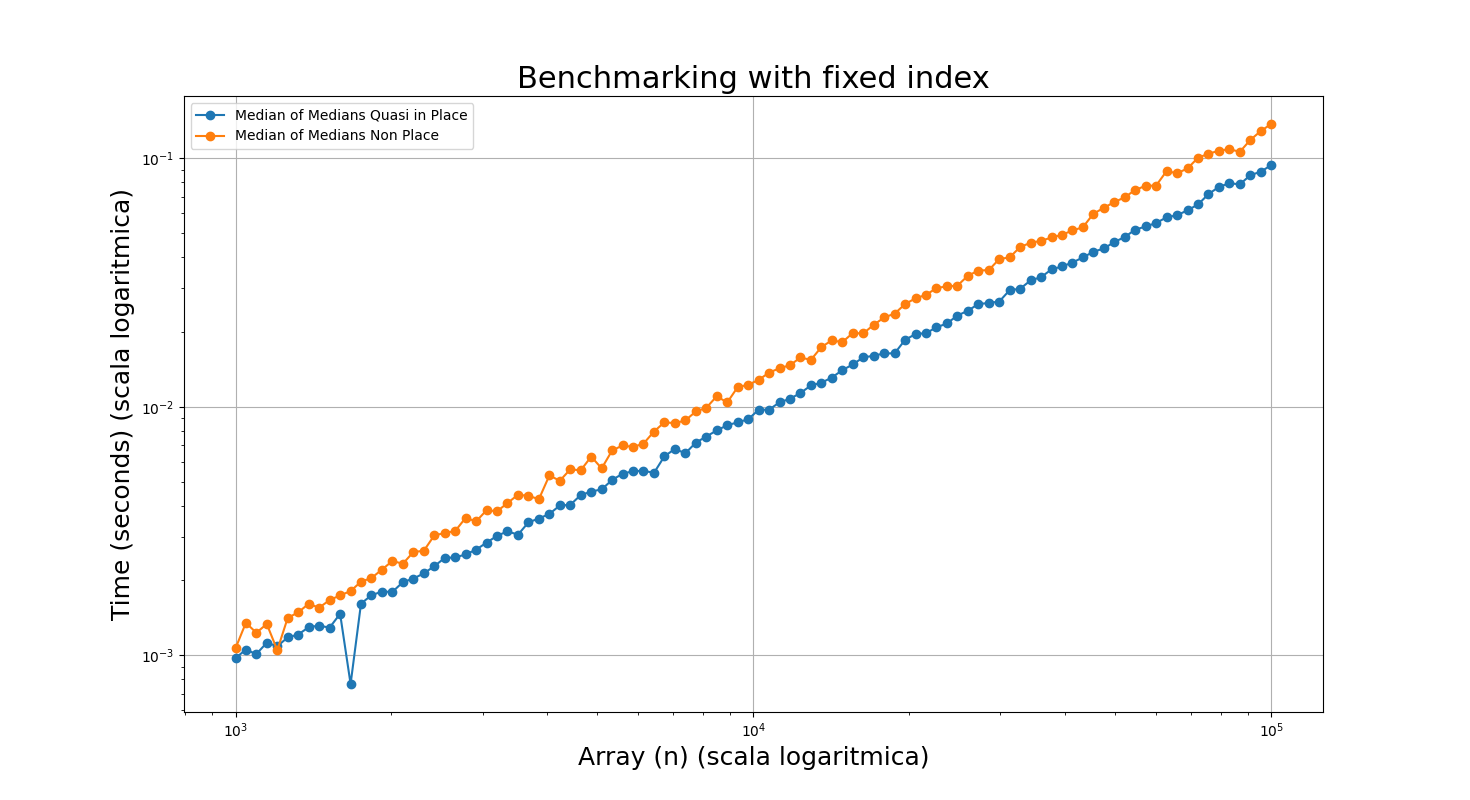
\includegraphics[width=.83\textwidth]{graphs/MoMs_2xlog.png}
\end{figure}

Dal grafico logaritmico notiamo che i due andamenti sono paralleli, come ci si aspetta, essendo la complessità temporale  $O(n)$ indipendentemente da come vengono memorizzate le mediane.
Dal grafico lineare vediamo poi che i tempi di esecuzione dei due algoritmi non si discostando, per cui possiamo concludere che il riutilizzo dello spazio non porta ad alcuna penalità nelle prestazioni.

\section{Conclusione}
Dall'analisi fatta nella sezione precedente possiamo trarre le seguenti conclusioni:
\begin{itemize}
	\item \QuickSelect{} risulta essere l'algoritmo più efficiente eccetto nel suo caso peggiore.
		Ciò è dovuto al basso overhead richiesto per la selezione del pivot.
		Al netto del caso peggiore è un buon candidato come algoritmo di selezione.
	\item \HeapSelect{} è un buon algoritmo quando $k$ è vicino agli estremi, ma la sua complessità nel caso in cui $k$ sia una frazione della dimensione dell'input lo rende peggiore degli altri due algoritmi analizzati.
		Inoltre se $k$ varia molto durante successive selezioni le prestazioni di \HeapSelect{} tendono a essere instabili.
	\item \MoMSelect{} è l'unico algoritmo con una complessità ottimale nel caso peggiore, ma l'overhead dovuto alla selezione del pivot lo rende meno efficiente di \QuickSelect{} in pratica.
		Contrariamente a \HeapSelect{} le sue prestazioni rimangono stabili al variare di $k$.
\end{itemize}

\end{document}
